%%
%% This is file `sample-sigconf.tex',
%% generated with the docstrip utility.
%%
%% The original source files were:
%%
%% samples.dtx  (with options: `sigconf')
%% 
%% IMPORTANT NOTICE:
%% 
%% For the copyright see the source file.
%% 
%% Any modified versions of this file must be renamed
%% with new filenames distinct from sample-sigconf.tex.
%% 
%% For distribution of the original source see the terms
%% for copying and modification in the file samples.dtx.
%% 
%% This generated file may be distributed as long as the
%% original source files, as listed above, are part of the
%% same distribution. (The sources need not necessarily be
%% in the same archive or directory.)
%%
%%
%% Commands for TeXCount
%TC:macro \cite [option:text,text]
%TC:macro \citep [option:text,text]
%TC:macro \citet [option:text,text]
%TC:envir table 0 1
%TC:envir table* 0 1
%TC:envir tabular [ignore] word
%TC:envir displaymath 0 word
%TC:envir math 0 word
%TC:envir comment 0 0
%%
%%
%% The first command in your LaTeX source must be the \documentclass command.
\title{Practical Course: Cloud Database Final Report}
\newcommand{\mytitle}{Practical Course: Cloud Database Final Report}
\documentclass[sigconf]{acmart}
\usepackage{fancyhdr}
\settopmatter{printacmref=false} % Removes citation information below abstract
\renewcommand\footnotetextcopyrightpermission[1]{} % removes footnote with conference information in first column

% 在模板加载后重新定义页眉
\AfterEndPreamble{
    \pagestyle{fancy}
    \fancyhf{} % remove header and foodnote
    \fancyhead[R]{\mytitle{} | \thepage} 
}

%% \BibTeX command to typeset BibTeX logo in the docs
\AtBeginDocument{%
  \providecommand\BibTeX{{%
    Bib\TeX}}}

%% Rights management information.  This information is sent to you
%% when you complete the rights form.  These commands have SAMPLE
%% values in them; it is your responsibility as an author to replace
%% the commands and values with those provided to you when you
%% complete the rights form.

% \setcopyright{}
% \copyrightyear{}
% \acmYear{2023}
% \acmDOI{}

%% These commands are for a PROCEEDINGS abstract or paper.
% \acmConference[Conference acronym 'XX]{Make sure to enter the correct
%   conference title from your rights confirmation emai}{June 03--05,
%   2018}{Woodstock, NY}
% \acmPrice{15.00}
% \acmISBN{978-1-4503-XXXX-X/18/06}


%%
%% Submission ID.
%% Use this when submitting an article to a sponsored event. You'll
%% receive a unique submission ID from the organizers
%% of the event, and this ID should be used as the parameter to this command.
%%\acmSubmissionID{123-A56-BU3}

%%
%% For managing citations, it is recommended to use bibliography
%% files in BibTeX format.
%%
%% You can then either use BibTeX with the ACM-Reference-Format style,
%% or BibLaTeX with the acmnumeric or acmauthoryear sytles, that include
%% support for advanced citation of software artefact from the
%% biblatex-software package, also separately available on CTAN.
%%
%% Look at the sample-*-biblatex.tex files for templates showcasing
%% the biblatex styles.
%%

%%
%% The majority of ACM publications use numbered citations and
%% references.  The command \citestyle{authoryear} switches to the
%% "author year" style.
%%
%% If you are preparing content for an event
%% sponsored by ACM SIGGRAPH, you must use the "author year" style of
%% citations and references.
%% Uncommenting
%% the next command will enable that style.
%%\citestyle{acmauthoryear}



%%
%% end of the preamble, start of the body of the document source.
\begin{document}

%%
%% The "title" command has an optional parameter,
%% allowing the author to define a "short title" to be used in page headers.
% \title{Practical Course: Cloud Database Final Report}

%%
%% The "author" command and its associated commands are used to define
%% the authors and their affiliations.
%% Of note is the shared affiliation of the first two authors, and the
%% "authornote" and "authornotemark" commands
%% used to denote shared contribution to the research.
\author{Weijian Feng}
\affiliation{%
  \institution{Technical University Of Munich}
  \streetaddress{15 Boltzmannstraße}
  \city{Munich}
  \country{Germany}}
\email{wj.feng@tum.de}

\author{Mingrun Ma}
\affiliation{%
  \institution{Technical University Of Munich}
  \streetaddress{15 Boltzmannstraße}
  \city{Munich}
  \country{Germany}}
\email{mingrun.ma@tum.de}

\author{Jingyi Jia}
\affiliation{%
  \institution{Technical University Of Munich}
  \streetaddress{15 Boltzmannstraße}
  \city{Munich}
  \country{Germany}}
\email{jingyi.jia@tum.de}

%%
%% By default, the full list of authors will be used in the page
%% headers. Often, this list is too long, and will overlap
%% other information printed in the page headers. This command allows
%% the author to define a more concise list
%% of authors' names for this purpose.
% \renewcommand{\shortauthors}{Trovato et al.}

%%
%% The abstract is a short summary of the work to be presented in the
%% article.
\begin{abstract}

Designing a NoSql distributed databases faces lots of challenges. In this paper we will introduce design methodology via Java of our project. We will also introduce benchmarking tests we have done in order to find out the limitation of database so that it can be further improved.

\end{abstract}

%%
%% The code below is generated by the tool at http://dl.acm.org/ccs.cfm.
%% Please copy and paste the code instead of the example below.
%%
\begin{CCSXML}
<ccs2012>
   <concept>
       <concept_id>10002951.10002952.10003190.10010832</concept_id>
       <concept_desc>Information systems~Distributed database transactions</concept_desc>
       <concept_significance>300</concept_significance>
       </concept>
   <concept>
       <concept_id>10002951.10002952.10003190.10003193.10003429</concept_id>
       <concept_desc>Information systems~Database recovery</concept_desc>
       <concept_significance>300</concept_significance>
       </concept>
 </ccs2012>
\end{CCSXML}

\ccsdesc[300]{Information systems~Distributed database transactions}
\ccsdesc[300]{Information systems~Database recovery}

%%
%% Keywords. The author(s) should pick words that accurately describe
%% the work being presented. Separate the keywords with commas.
\keywords{No-Sql database, KV database, transaction, consistent hashing}
%% A "teaser" image appears between the author and affiliation
%% information and the body of the document, and typically spans the
%% page.

%%
%% This command processes the author and affiliation and title
%% information and builds the first part of the formatted document.
\maketitle

\section{Introduction}

In the ever-evolving landscape of digital applications, where the demand for seamless user experiences, vast data handling, and continuous availability reigns supreme, the architecture that underpins these systems must evolve as well. This evolution is particularly evident in the realm of large-scale web-based applications, which cater to millions of online users concurrently. To effectively manage the colossal influx of data and ensure uninterrupted service, traditional database management systems, while robust and versatile, often fall short in meeting the specialized requirements of such dynamic and demanding environments.

The significance of key-value stores transcends mere adaptation; it entails a conceptual shift from the conventional ACID (Atomicity, Consistency, Isolation, Durability) transaction model, towards a more agile and performance-oriented approach encapsulated by the BASE model (Basically Available, Soft state, Eventually consistent). This transition, while introducing an intentional trade-off between consistency and performance, becomes the cornerstone upon which efficient and reliable database scalability is erected. With the BASE model as its foundation, the key-value store architecture opens the door to data distribution and replication across an array of powerful servers, thereby setting the stage for a new era of resilient and scalable distributed storage systems.

The objective of this essay is to delve into the intricacies of extending the centralized storage server architecture, transforming it into a sharded, load-balanced system – a system capable of accommodating vast amounts of data by harnessing the principles of consistent hashing. This technique empowers the distribution of data records, manifested as key-value pairs, across a network of storage servers. Each server takes ownership of a distinct portion of the data space, strategically aligned with a continuous range of hash values. The orchestration of this distributed landscape relies on the discerning application of hash functions to precisely pinpoint the location of specific data tuples, contingent upon the hash value associated with the respective key.

Throughout this essay, we will navigate the intricacies of this evolved NoSQL distributed storage system, exploring its architectural components, mechanisms, and challenges. By delving into the principles of consistent hashing, the dynamics of metadata management, and the role of the Elastic Control Service, we aim to unveil a comprehensive understanding of how the centralized storage server architecture has metamorphosed into a robust, adaptable, and scalable distributed storage solution.


% ACM's consolidated article template, introduced in 2017, provides a
% consistent \LaTeX\ style for use across ACM publications, and
% incorporates accessibility and metadata-extraction functionality
% necessary for future Digital Library endeavors. Numerous ACM and
% SIG-specific \LaTeX\ templates have been examined, and their unique
% features incorporated into this single new template.

% If you are new to publishing with ACM, this document is a valuable
% guide to the process of preparing your work for publication. If you
% have published with ACM before, this document provides insight and
% instruction into more recent changes to the article template.

% The ``\verb|acmart|'' document class can be used to prepare articles
% for any ACM publication --- conference or journal, and for any stage
% of publication, from review to final ``camera-ready'' copy, to the
% author's own version, with {\itshape very} few changes to the source.

\section{Problem Statement}
Creating a distributed NoSQL database system that seamlessly integrates transactional consistency and sharding introduces a multifaceted set of challenges, requiring careful consideration of the following dimensions:

1. \textbf{Consistency and Isolation in Transactions}: Maintaining transactional integrity across a distributed NoSQL system, where data is spread across multiple nodes, poses a significant challenge. Ensuring the ACID properties (Atomicity, Consistency, Isolation, Durability) in a distributed environment, while allowing for high-performance operations, requires innovative mechanisms to coordinate and manage transactions.

2. \textbf{Sharding Strategies and Data Distribution}: Sharding involves partitioning the dataset across multiple nodes to enable horizontal scalability. Designing effective sharding strategies that distribute data optimally while minimizing data skew, hotspots, and imbalances is a complex endeavor. Ensuring that related data is appropriately co-located to support efficient queries adds another layer of complexity.

3. \textbf{Transactional Consistency Across Shards}: In a sharded environment, ensuring consistency across transactions that involve data across different shards is a challenge. Coordinating distributed transactions and maintaining global consistency, even in the presence of node failures or network partitions, requires sophisticated protocols and strategies.

4. \textbf{Concurrency and Isolation in Sharded Transactions}: Sharded systems introduce the challenge of managing concurrent transactions across multiple shards. Ensuring isolation levels and preventing conflicts, while allowing for efficient parallelism, demands robust coordination mechanisms and careful handling of potential anomalies.

5. \textbf{Failure Recovery and Resilience}: Distributed systems are prone to various types of failures, such as node crashes or network partitions. Designing strategies to detect failures, recover from them, and maintain system availability without compromising data integrity is crucial.

6. \textbf{Dynamic Scaling and Shard Migration}: The ability to dynamically scale the system by adding or removing nodes introduces the challenge of managing shard migrations. Developing algorithms and protocols to handle migration efficiently, without causing service disruptions or degraded performance, is essential.

7. \textbf{Metadata Management}: Sharded systems require metadata management to track the location of data across shards and ensure proper routing of queries. Developing strategies to maintain accurate and up-to-date metadata without introducing performance bottlenecks is challenging.

8. \textbf{Trade-off between Consistency and Performance}: Balancing the need for transactional consistency with the desire for high-performance operations can be intricate. Designing mechanisms that allow applications to choose appropriate consistency levels for different scenarios while maintaining acceptable performance is a delicate task.
\section{Approach}

\subsection{Network I/O}

During the communication between the ECS registry center and the KVServer servers, their roles will be exchanged once.

The ECS registry center uses a BIO thread pool to provide registration services externally. It starts before all other KVServer nodes and waits for connections from KVServer nodes on a specific IP:Port. When a KVServer node connects, ECS will spawn a dedicated thread to handle the offline work of the KVServer node and then act as a client of the KVServer by constructing an NIO SocketChannel connection to the KVServer. This is followed by metadata synchronization, data transfer, and other operations.

There are two types of I/O communication in KVServer. When a KVServer comes online, it first builds a BIO socket to register with the ECS. At this time, the KVServer acts as a client of the ECS. After registration, when the KVServer acts as a server to provide services externally, it adopts the Java NIO communication mode. We consolidate the requests from ECS and the requests from clients connected to the KVServer into the NIO next.isReadable() detection state. At this point, ECS's role is transformed into a client of the KVServer.

Java NIO is an I/O model provided by Java, introducing a set of new APIs for efficient multiplexed I/O operations. Compared to traditional Java BIO, Java NIO provides a more flexible and high-performance way to perform I/O operations.

The core components of Java NIO include the following:

1. Channel: A channel is the conduit for data transfer and can be used to read and write data. Java NIO provides different types of channels, such as file channels and socket channels.
2. Buffer: A buffer is an object used to store data and enables reading and writing data. Buffers provide a structured way to access data based on different data types (e.g., bytes, characters).
3. Selector: A selector is a mechanism for multiplexing non-blocking channels. It manages multiple channel I/O operations in a single thread. The selector can listen to events on multiple channels and handle them accordingly when events occur.

\subsection{Data Storage}

\subsubsection{Data Persistence}

Data persistence is the process of storing data in non-volatile media (such as hard drives, solid-state drives, flash storage) to ensure data is retained and can be recovered and used after a computer system shutdown or power failure, without data loss.

For this project, considering the small scale of data, we have adopted a simple data persistence solution, which stores each key-value pair in a corresponding file to achieve data persistence.

To improve the efficiency of read and write operations, we have implemented a dual-database architecture: the main database and the backup database. The backup database is stored only on the hard disk and is typically not accessed externally. The main database is stored both on the hard disk and in the cache. When a client writes data, the data is first written to the main data cache and then asynchronously copied to the hard disk directory of the main database and backup database. When performing read operations, the system first checks the main data cache, and if the data is not found in the cache, it queries the data on the hard disk.

With this architecture, we can achieve data persistence and improve the efficiency of read and write operations. The presence of the backup database serves as redundant backup to provide higher data reliability. At the same time, the caching mechanism of the main database speeds up data retrieval and improves system response time.

\subsubsection{Cache Update Strategy}

Regarding the replacement strategy for key-value pairs in the cache, the following three strategies can be implemented:

1. First-In-First-Out (FIFO): Key-value pairs that enter the cache first will be replaced based on the order of entry.
2. Least Recently Used (LRU): Key-value pairs that have been least recently used, based on their access time, will be replaced. We use Java's LinkedHashMap to implement the LRU strategy, where the most recently accessed key-value pairs are kept at the head of the linked list. When the cache is full, the key-value pair at the tail of the list is replaced.
3. Least Frequently Used (LFU): Key-value pairs that have been least frequently used, based on their access frequency, will be replaced. We use a hash table combined with a priority queue to implement the LFU strategy, tracking and managing key-value pairs and their corresponding access frequencies. When the cache is full, the key-value pair with the lowest access frequency is replaced.

When a GET request from the client leads to a cache miss, the corresponding key-value pair will be searched on the disk and moved to the cache. If the cache is full, based on the currently selected strategy, a specific key-value pair will be selected for replacement and swapped to the disk (which may involve updates on the disk). Similarly, when a PUT request is received from the client and the cache is full, a specific key-value pair will be selected for replacement based on the selected strategy.


%%%%%%%%%%%%%%%%%%%%%%%%%%%%%%%%%%%%%%%%%%%%%%%%%%%%%%%%%%%%%%%%%%%%%%%%%%%%
\section{Architecture}
\begin{figure}[htbp]
    \centering
    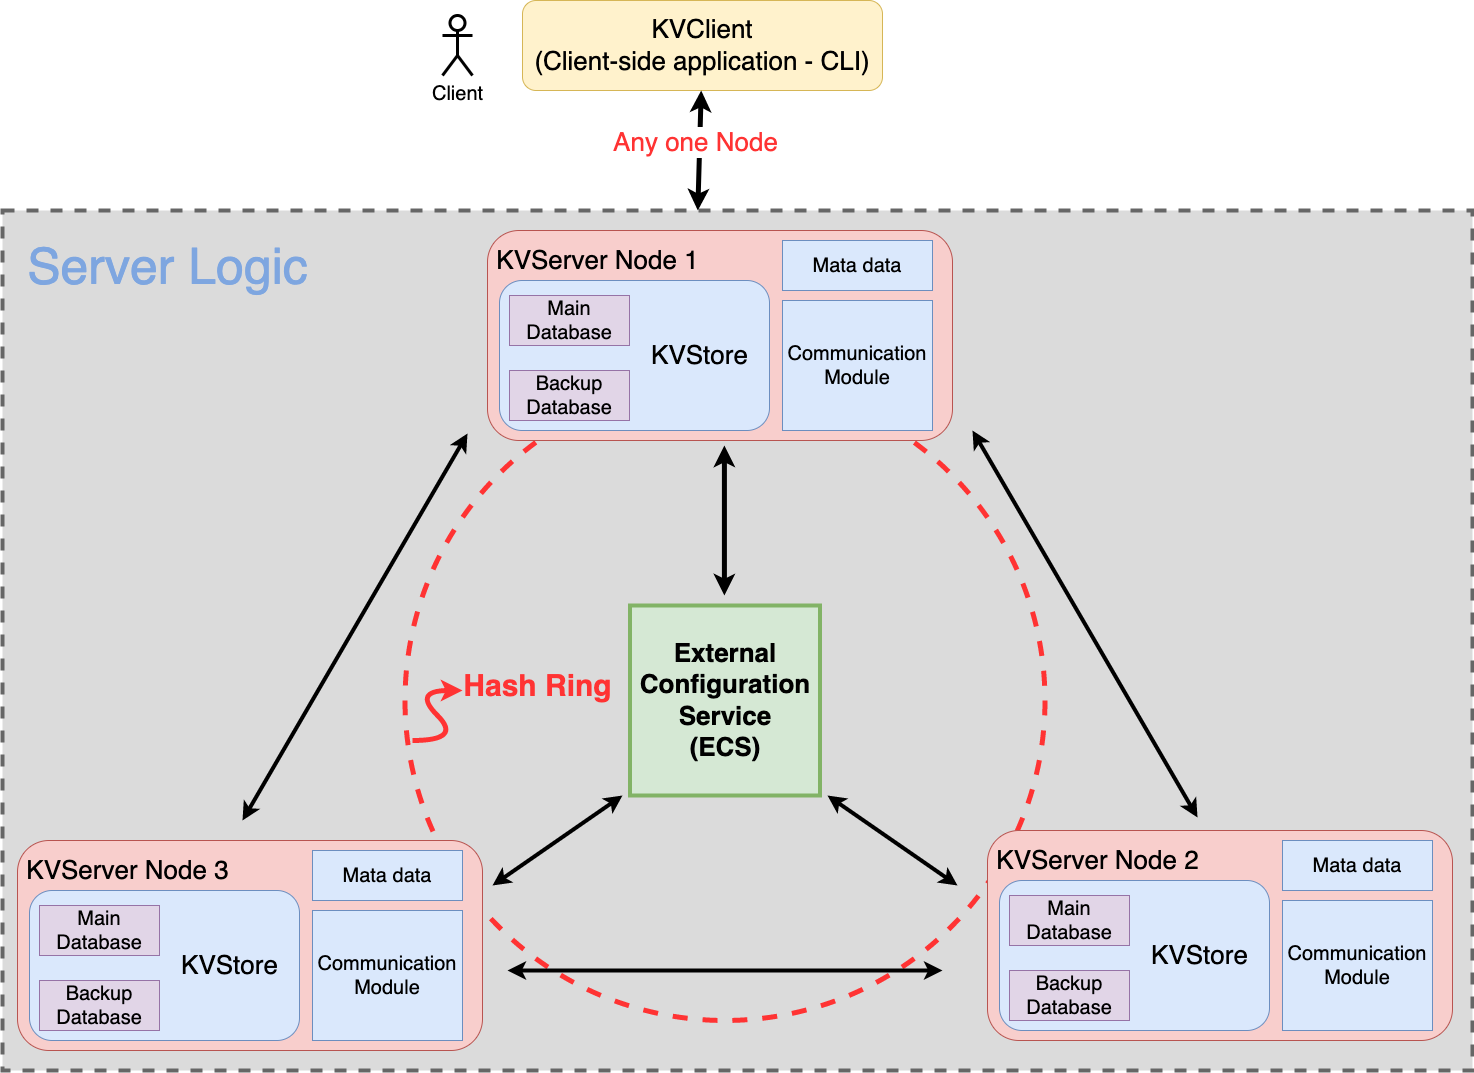
\includegraphics[width=0.5\textwidth]{cloud_database_report/asset/overview.png}
    \caption{Overivew of the Distributed Cluster}
    \label{fig:xxx}
\end{figure}
Components
\begin{itemize}
    \item Registry Center: Cluster management
    \item KVServer: Server nodes
    \begin{itemize}
        \item KVStore: Database
    \end{itemize}
\end{itemize}

\subsection{Bootstrap Server Registry}

In distributed systems, a bootstrap server refers to a special server used to bootstrap (initialize) new nodes joining the system or remove nodes that need to be taken offline. It serves as a central node for managing various nodes in the hash ring and plays a crucial role, including updating the hash ring, guiding data migration among nodes, and monitoring the status of all nodes. By having a bootstrap server and its functionality, distributed systems can manage the process of node joining and exiting more stably and reliably, optimize data distribution and access efficiency, and provide a high-performance and scalable system architecture.


\subsubsection{Adding a KVServer}
When a new KVServer connects to ECS, the following operations are performed:
\begin{itemize}
    \item Determine the position of the new storage server in the ring based on the server's port address used for communication with clients.
    \item Recalculate and update the hash ring.
    \item Initialize the new storage server using the updated hash ring.
    \item Set write locks on successor nodes.
    \item Data transfer: Transfer affected data items to the new storage server.
    \item Once all affected data has been transferred, send the updated hash ring to all storage servers.
\end{itemize}

\subsubsection{Removing a KVServer}
When a KVServer sends a removal notification to ECS or ECS detects a node failure, the following operations are performed:
\begin{itemize}
    \item Add the node to the removal queue in ECS and process them one by one.
    \item Recalculate and update the hash ring.
    \item Data transfer: Transfer affected data items to new storage servers.
    \item Once all affected data has been transferred, send the updated hash ring to the remaining storage servers.
    \item Continue shutting down the storage server.
\end{itemize}

\subsubsection{Monitoring the status of KVServer}
ECS assigns a dedicated thread to periodically monitor if servers go offline. Specifically, when \texttt{socket.isclose()} is true, it indicates the server is offline, and the appropriate logic for handling the offline event is invoked.


\subsection{Cluster Communication}

Cluster communication refers to the process of mutual communication and collaboration between multiple nodes in a distributed system through the network. In cluster communication, nodes can be physical servers, virtual machines, containers, etc., connected through the network to enable data transfer, task allocation, coordination, synchronization, and other operations.

In the context of cluster communication, we have implemented two distinct schemes: one employs JSON, while the other leverages the gRPC (gRPC Remote Procedure Call) framework.

In our implementation based on JSON, we use custom string messages for cluster communication. Each message is encoded and decoded as a string and transmitted to other nodes through the network. We use a message builder factory to generate message instances, creating corresponding message objects based on the message type and related data. This allows dynamic generation of different types of messages to meet the requirements of cluster communication.

To handle received messages, we use a unified message parser. The message parser is responsible for parsing received string messages and executing corresponding operations based on the message format and rules. This ensures consistency in message handling and improves code readability and maintainability.

In contrast to the JSON-based approach, the implementation using the gRPC framework offers a more structured and efficient way of achieving cluster communication. gRPC is a high-performance open-source framework that facilitates remote procedure calls (RPCs) across different nodes in a distributed system. Unlike the custom JSON messages, gRPC uses protocol buffers (protobufs) to define the service interface and message formats in a language-agnostic manner. With gRPC, communication is driven by service method calls. Each method call corresponds to a specific operation that can be executed on a remote node. The gRPC framework handles the underlying network communication, serialization, and deserialization of messages, making it a more efficient and reliable choice for cluster communication compared to the custom JSON-based approach.

Please refer to the API documentation for specific communication protocols.

\subsection{Transaction}
We use Two-Phase Commit (2PC)\cite{lampson1979crash} \cite{fan20202pc} and Two-Phase Locking (2PL) \cite{lin1983basic}\cite{barthels2019strong} to ensure the atomicity, consistency, isolation, and durability of database operations, thereby ensuring data correctness and reliability.

When implementing transactions using the Two-Phase Commit (2PC) protocol, coordination occurs between a Transaction Coordinator and Participants. The process involves two phases:

\begin{itemize}
    \item \textbf{Prepare Phase}: The Transaction Coordinator sends a prepare request to all Participants, asking if they are ready to commit the transaction. Participants perform their corresponding operations and respond with information about their preparedness.
    
    \item \textbf{Commit Phase}: If all Participants are prepared, the Transaction Coordinator sends a commit request, instructing all Participants to commit the transaction. Participants receive the commit request, execute the actual commit operation, and send back a message confirming the completion of the commit.
\end{itemize}

Through these two phases, the Transaction Coordinator ensures that either all Participants have successfully committed the transaction or all have rolled back the transaction, thereby maintaining transaction consistency and isolation.

In the context of the Two-Phase Locking (2PL) protocol, transaction execution involves two phases:

\begin{itemize}
    \item \textbf{Locking Phase}: The transaction initially acquires all required locks. During this phase, the transaction can acquire locks but cannot release them.
    
    \item \textbf{Unlocking Phase}: Once the transaction has acquired all necessary locks, it begins executing database operations. After completing its operations, the transaction releases the locks it holds.
\end{itemize}


\subsection{Load Balancing}

Load balancing \cite{ghomi2017load} \cite{chou1982load} is a technique that distributes the workload, such as network traffic, requests, or computing tasks, across multiple computing resources to improve system performance, reliability, and scalability. Load balancing ensures that each computing resource is utilized properly, avoids resource overload, and enhances system fault tolerance.

Consistent hashing algorithm \cite{coluzzi2023survey} \cite{karger1997consistent} is applied to our distributed system to address load balancing and node expansion requirements. We plan to introduce virtual nodes in the future.

Consistent hashing is an algorithm used to solve the load balancing problem \cite{wang2007load}. Traditional hashing algorithms map resources and requests to a fixed hash table. However, in a distributed environment, when the number of nodes changes, a large number of remappings occur, which negatively affects the stability and performance of the system.

Consistent hashing algorithm maps resources and requests to a hash ring, represented as a circular structure. Each resource node has a corresponding position on the ring, and requests are mapped to the nearest resource node based on a hash function. When a new request arrives, the consistent hashing algorithm maps it to the resource node closest to its position.

Consistent hashing solves the issue of remapping a large portion of requests when nodes change in traditional hashing algorithms. When a node is added or removed from the system, only requests in the vicinity of that node are affected, while the mapping relationship between other nodes and requests remains unchanged. By adjusting the positions of nodes on the ring, the impact of adding or removing nodes is minimized.

As shown in the diagram, consistent hashing effectively handles node scaling up or down.
\begin{figure}[htbp]
    \centering
    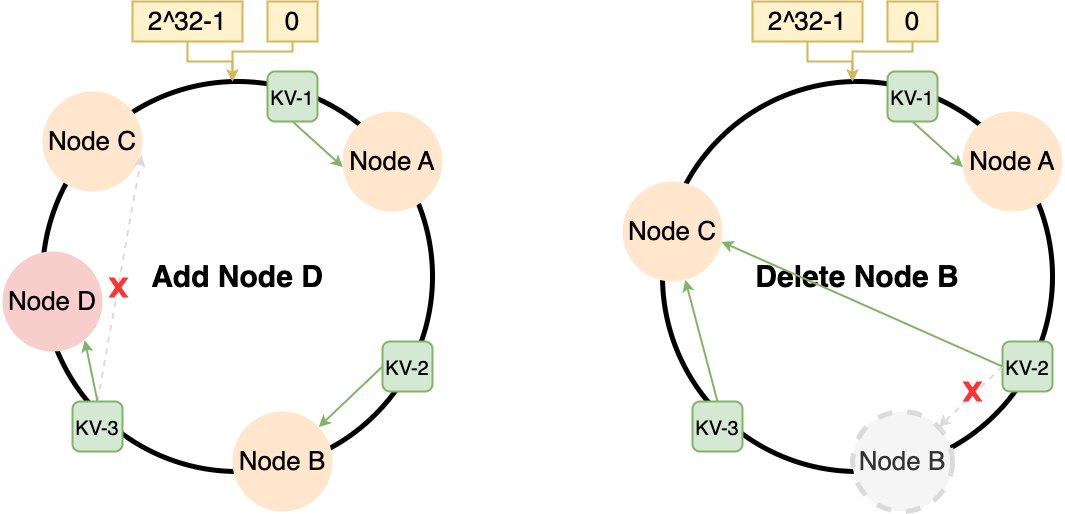
\includegraphics[width=0.5\textwidth]{cloud_database_report/asset/consisten.png}
    \caption{Consistent Hashing}
    \label{fig:xxx}
\end{figure}

To further improve system scalability and fault tolerance, we plan to extend our distributed system to support virtual nodes in the future. Virtual nodes will be mapped to physical nodes and enable finer-grained distribution of data and requests, further enhancing load balancing effectiveness.


\subsection{Fault Tolerance}

Fault tolerance\cite{jalote1994fault} is the ability of a distributed system to handle node failures or errors, ensuring system availability and reliability. It aims to enable the system to continue normal operation in the event of node failures and minimize the impact on users as much as possible through backup mechanisms, fault detection, and recovery strategies.

Selection of Backup Nodes: In our implementation, we have chosen a simple and effective backup strategy, which designates the previous node on the hash ring as the backup node for each current node. This means that each node has a backup node to store the same data replica.

Backup Node Data Synchronization: When a write request occurs, we asynchronously propagate the data update to the backup node. Specifically, when a write request arrives at the current node, we first write the data to the storage of the current node and then asynchronously pass the same write operation to the backup node to maintain data eventual consistency. (See AP eventual consistency)

Fault Detection and Recovery: In our implementation, we use polling to detect node disconnections. We periodically poll the connection status of each thread to quickly detect node failures. Once a failure is detected, the central node adds the faulty node to the pending removal node list and processes each node in the list: remove the node from the hash ring and update the hash ring of all nodes. Additionally, since we use a backup node strategy based on the hash ring, the corresponding backup node automatically becomes responsible for the data and takes over the work of the failed node. This means that after a failure occurs, the system can continue to operate seamlessly.

We also plan to implement other fault detection and recovery strategies, such as heartbeat mechanism and fault recovery protocols, to further improve system reliability and fault tolerance.


\subsection{Consistency Guarantees}

In distributed systems, data is often replicated on multiple nodes to improve system availability and fault tolerance. When performing update operations on data, due to network latency, node failures, or concurrent operations, data replication may not be instantaneous. Therefore, different nodes in the system may have different data replicas during the data replication process. The eventual consistency model assumes that, without new update operations, after a period of synchronization and data exchange, the system will eventually reach a consistent state. This means that if no new write operations occur, all nodes in the system will eventually converge to the same data replica.

In this system, CompletableFuture is used for asynchronous replication, which has the advantages of low latency and high performance. However, it also introduces some issues.

Our cluster cannot guarantee strong consistency. Although strong consistency is generally ensured in most cases, there is a possibility of data loss in an extreme scenario: if a client writes some data, the master node confirms the write, but before propagating the newly written data to any replica and successfully flushing it to the disk, the master crashes. As a result, the write is permanently lost.

Improving consistency can be achieved by forcing the database to flush data to the disk before replying to the client, but this often leads to low performance. Therefore, it is a trade-off between performance and consistency.



%%%%%%%%%%%%%%%%%%%%%%%%%%%%%%%%%%%%%%%%%%%%%%%%%%%%%%%%%%%%%%%%%%%%%%%%%%%
\section{Evaluation}
In this section, we present a comprehensive evaluation of the proposed two cloud database system (the system based on JSON and the system based on gRPC), focusing on their performance and query optimization capabilities. We conducted a series of experiments to assess the systems' efficiency in handling various workloads and their ability to provide timely responses to user queries. The evaluation aims to validate the effectiveness of our system's architecture and design decisions.

\subsection{Experiment Setup}
To simulate a distributed environment, we conducted a series of experiments using a single machine to represent a 3-node cluster. Specifically, we employed our system on MacBook M1 with 8-core CPU M1 chip and 8 GB RAM. Additionally, Apache JMeter is utilized to load test functional behavior and measure performance.  The following steps outline our setup process: \\
\textbf{1. Thread Group Definition\\ }
We created two Thread Groups within JMeter, representing two different workload scenarios: put key-value into the databases and get data from them. Each Thread Group was configured to run a certain number of threads concurrently to simulate user interactions.\\
\textbf{2. Number of Threads and Ramp-Up Period\\}
We adjusted the number of threads in each Thread Group to imitate different levels of user activity. In this test, where we wanted to see the maximum capacity of our system, we gradually increased the number of threads (which represent users) from 1 to 500. We also set a 200-second period for each Thread Group, during which new threads were introduced, mimicking how real users join over time. To make sure we had a consistent load, we allowed each thread to exist for 250 seconds, ensuring that we always had 1000 threads active.\\
\textbf{3. Requests and Workload Composition\\ }
Within each Thread Group, we defined specific TCP requests representing different database operations, including PUT and GET operations. We use random generated key-value pairs as our test dataset.\\
\textbf{4. Results Collection and Analysis\\}
We configured JMeter to collect various performance metrics during the experiments, including throughput, latency, and resource utilization. These metrics provided insights into how the system behaved under different workload conditions.

\subsection{Performance Metrics}
We measured the performance of our database system using the following metrics:
\begin{itemize}
    \item {\texttt{Throughput}}: The time taken to respond to a query.
    \item {\texttt{Latency}}: The time taken to respond to a query.
    \item {Error}: The number of failed requests.
\end{itemize}

\subsection{Results}
First we compare the performance of two different database system.  Figure \ref{fig:latnecy} and Figure \ref{fig:throughput} shows the performance different between system based on gRPC and the one based on JSON. Two observations we can be made from these figures. First, the database system that uses gRPC technology has much faster response times compared to the one that uses JSON. This is what we expected, as gRPC is known for being efficient. Second, both systems show similar levels of throughput. This means they handle a similar amount of work in a given time. This similarity might be because the testing machine we used has its own limitations, which prevent us from seeing a bigger difference in throughput between the two systems.
\begin{figure}
    \centering
    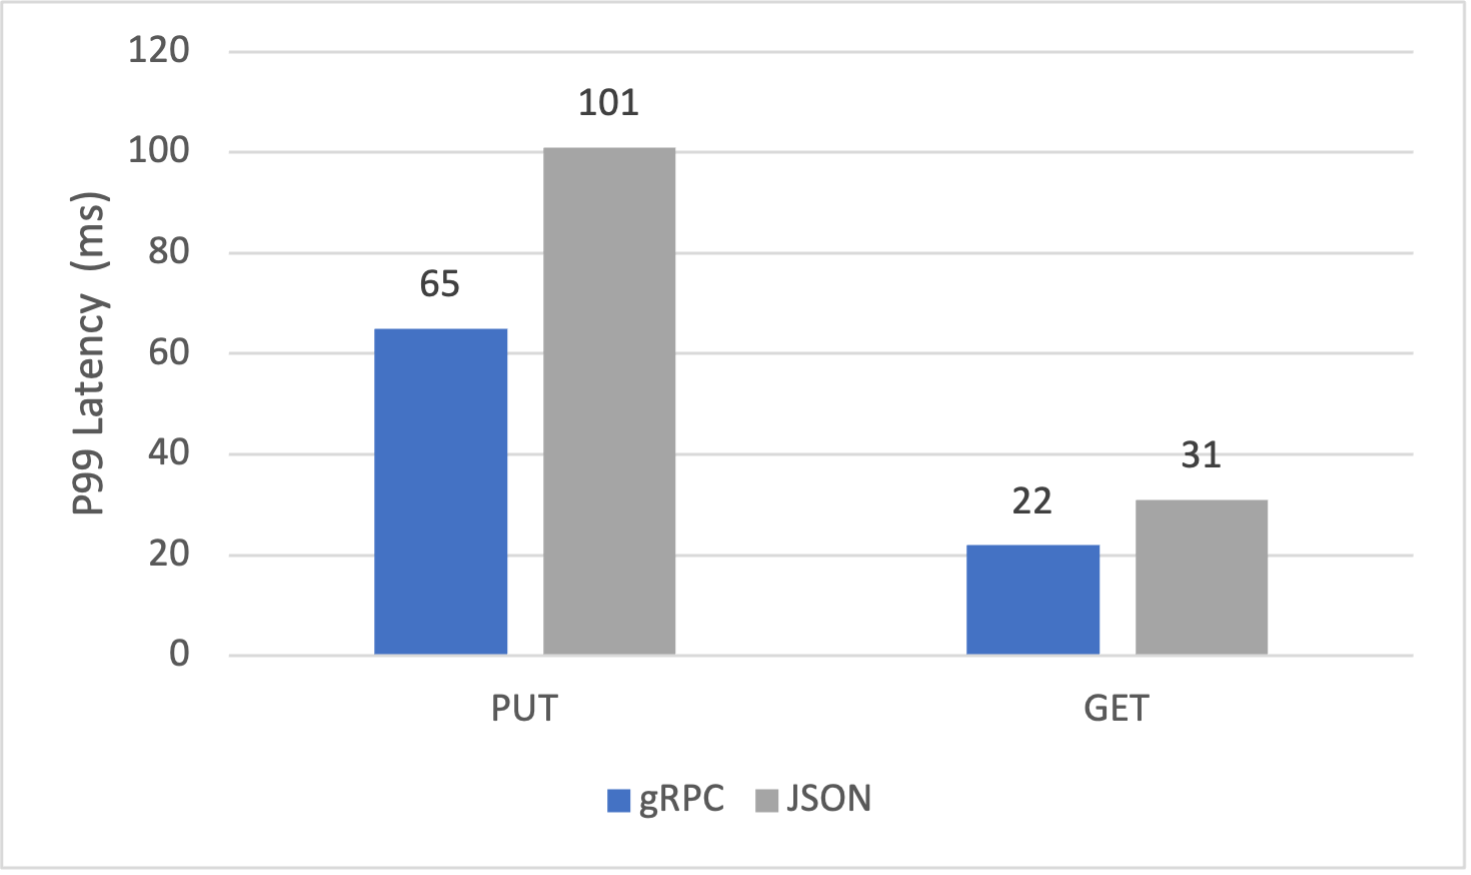
\includegraphics[width=1\linewidth]{latency.png}
    \caption{Compare the P99 Latency of two system}
    \label{fig:latnecy}
\end{figure}
\begin{figure}
    \centering
    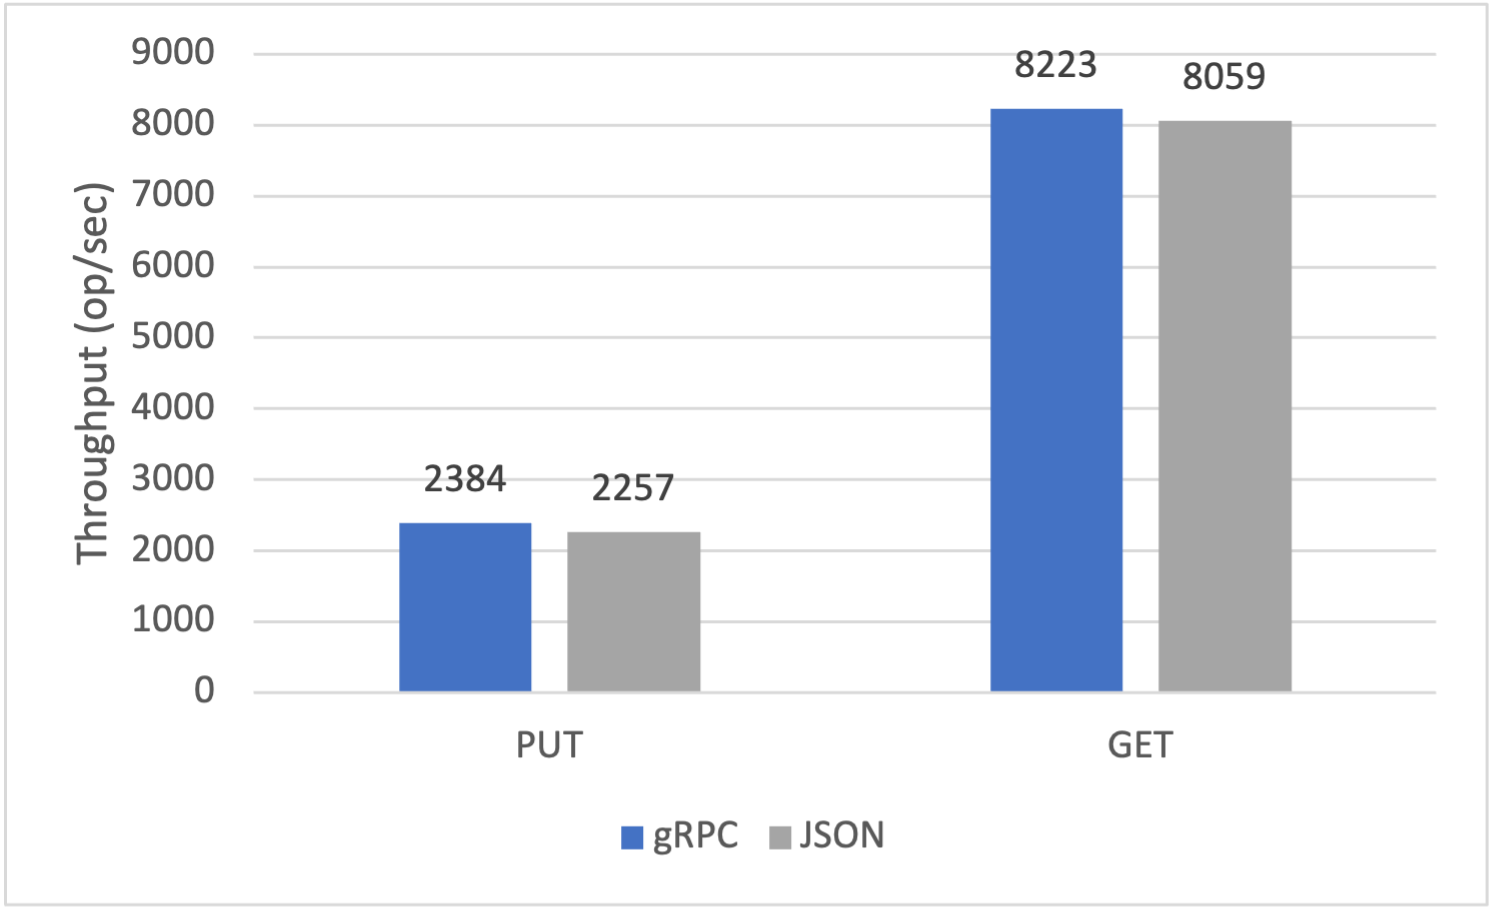
\includegraphics[width=1\linewidth]{throughput.png}
    \caption{Compare the throughput of two system}
    \label{fig:throughput}
\end{figure}

Then we focus on evaluating the performance of database system based on gRPC. To showcase the impact of different workloads on performance of it, Figure \ref{put} illustrates how the number of active threads relates to the average time it takes to receive a response for PUT requests. In a similar manner, Figure \ref{get} demonstrates this connection for GET requests. Clearly, in both cases, the time it takes for a response increases as more users connect. However, with PUT requests, we start to see more noticeable fluctuations in response time beyond around 250 users. This could be due to the system struggling to handle such a large number of users and causing instability.

Additionally, it's important to highlight that the response time for GET requests is significantly lower than that of PUT requests. This is because, in our system, every PUT request requires checking the database to see if a specific piece of information already exists, which takes a considerable amount of time.
\begin{figure}
    \centering
    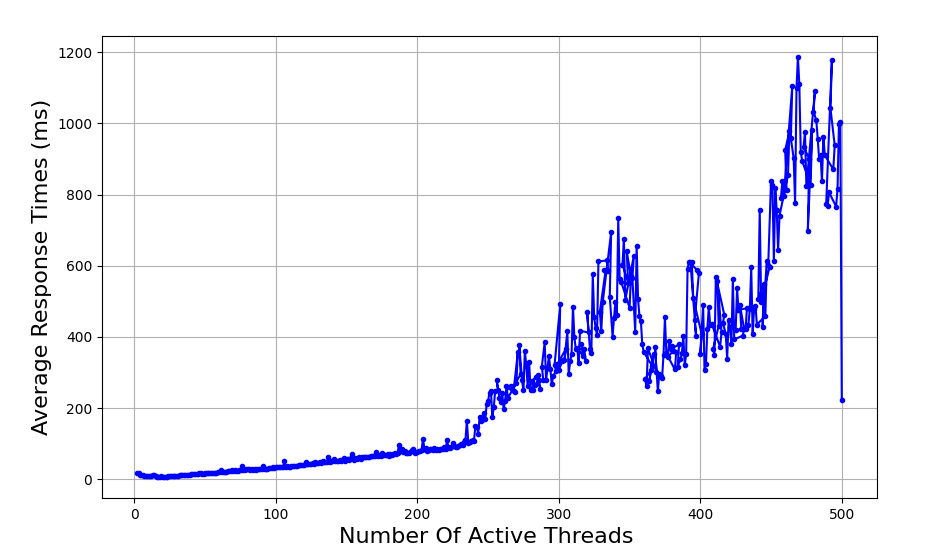
\includegraphics[width=1\linewidth]{cloud_database_report/report/put_time_thread.png}
    \caption{Analyzing the Relationship Between Active Thread Count and Average Response Time Of PUT Requests}
    \label{put}
\end{figure}
\begin{figure}
    \centering
    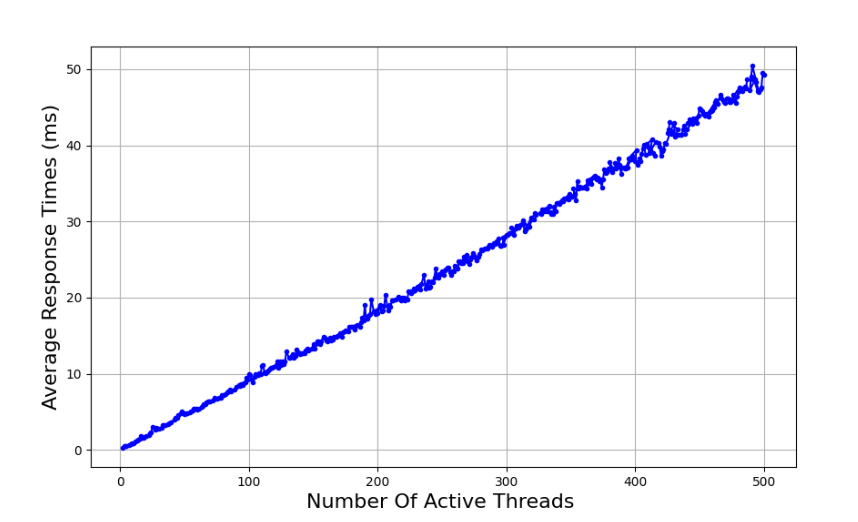
\includegraphics[width=1\linewidth]{get_time_thread.png}
    \caption{Analyzing the Relationship Between Active Thread Count and Average Response Time Of GET Requests}
    \label{get}
\end{figure}
\section{Conclusions}
\subsection{What we Learned}

During the development of this project, we had opportunities to implement theoretical knowledge in lectures like database system and distributed system and had to deal with lots of challenges. One of the most challenged topic is to ensure consistency because of sharding and meanwhile ensuring durability.

We also progressed our skills in dealing with real engineering or developing tasks and effectively coping with team-working by utilizing git and IntelliJ IDEA. We learned how to write unit test for Java code and how to use Java's benchmarking tool Jmeter.

Ability to design extendable programs is also improved during the process of 5 iterations of feature design. One important lesson is the possible future extensions or potential supportable features should taken into account during interface design. Otherwise to modify codes which are not easily extendable can be a huge burden in the future.

\subsection{Future Plans}

The single point of failure in ECS needs to be addressed by consensus algorithms like Raft or Paxos, which distribute the functionality of ECS directly among the servers. Implementing Raft or similar algorithms directly can be complex, so for now, an ECS registry center is abstracted to handle this task.

The current data persistence method is suitable for small-scale data. For large-scale data, we plan to adopt a tabular storage approach inspired by relational databases to store data.

Other isolation level, such as read-commited and repeatable read could be provided if they are needed.


%%
%% End of file `sample-sigconf.tex'.


%%
%% The next two lines define the bibliography style to be used, and
%% the bibliography file.
\bibliographystyle{ACM-Reference-Format}
\bibliography{sample-base}


%%
%% If your work has an appendix, this is the place to put it.
\appendix



\end{document}
\endinput
%%
%% End of file `sample-sigconf.tex'.
